% Provenance (never printed): old terminale S material on past climates (ice cores,
% pollen, ocean sediments and oxygen isotopes, glacial-interglacial cycles, the
% astronomical rhythm told, climates of deep time), read from data. Owner (Sync 0/1):
% climate archive and proxy, ice core, glacial period, interglacial and glacial cycle,
% pollen analysis, Last Glacial Maximum. Recalled: glacier, ice sheet, ice age (Book 1,
% grade 8); the first look at the ice-core records (Book 1, grade 9); isotopes
% (physics); greenhouse gases (chemistry); the time scale (Book 1, grade 7). The
% delta notation of isotopes is Book 3's: isotope curves are read here as told,
% without a definition. The orbital theory of climate belongs to a university book:
% told here only. Physical science only, in the IPCC's calibrated words.
% Figures: figdata/grade-12/ice_age_records.py (tests/grade-12/test_ice_age_records.py).
\chapter{Membaca Iklim Masa Lalu}\label{ch:g12:past-climates}

Di Dome~C, \qty{3233}{m} di atas permukaan laut pada lapisan es Antarktika
Timur, suhu udara rata-rata setahun sekitar \qty{-55}{\degreeCelsius}. Sebuah
bor yang bekerja di sana berhenti pada kedalaman \qty{3260}{m}, sekitar
\qty{15}{m} di atas batuan di bawah es. Es terdalam yang diangkatnya
mengandung gelembung-gelembung udara kecil yang berumur sekitar \num{800000}
tahun: sampel atmosfer dari masa jauh sebelum para petani pertama. Bab ini
membaca iklim masa lalu di dalam es, di dalam lumpur danau dan dasar samudra,
dan di dalam batuan, lalu menanyakan apa yang dikatakannya tentang masa kini.
% ledger: ipev:concordia, edc3:drilling, jouzel07:edc

\begin{omfigure}
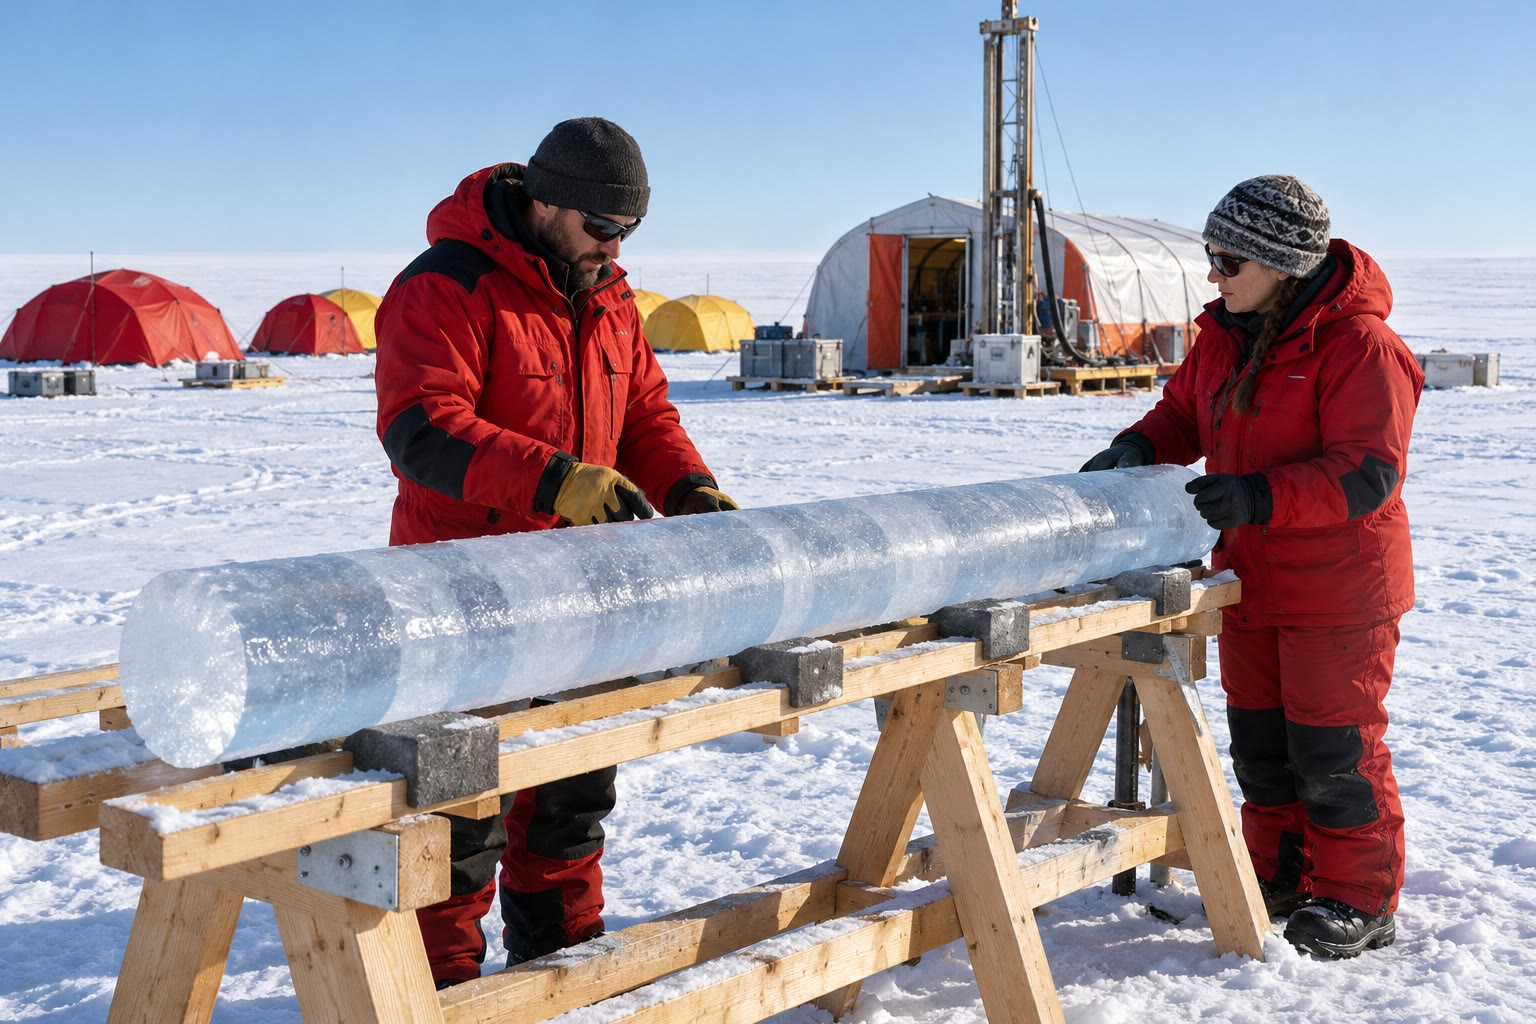
\includegraphics[width=0.56\linewidth]{images/book2/ai/g12-ice-coring-camp.jpg}

{\small Sebuah perkemahan pengeboran \omterm{def:g12:past-climates:ice-core}{inti es} di atas lapisan es kutub: bor bekerja
di bawah menara dan tempat berlindung, dan setiap potong inti dibentangkan,
dicatat, dan dikemas sebelum dikirim ke laboratorium (ilustrasi AI).}
\end{omfigure}

\begin{recall}
Gletser adalah massa es yang bertahan dari tahun ke tahun dan mengalir oleh
beratnya sendiri; lapisan es menutupi sebagian besar sebuah benua; zaman es
adalah masa dingin yang panjang ketika lapisan es menyebar jauh melampaui
kutub (Buku 1, kelas 8). Di dalam \omterm{def:g12:past-climates:ice-core}{inti es} Antarktika, salju merekam suhu udara
dan gelembung-gelembungnya menyimpan udara itu sendiri, dan kedua rekaman itu
naik dan turun bersama (Buku 1, kelas 9). Atom-atom satu unsur dapat berbeda
jumlah neutronnya: isotop-isotop ini berperilaku sama secara kimia tetapi
berbeda massanya (buku-buku fisika). Karbon dioksida adalah gas rumah kaca
(buku-buku kimia). Zaman Kuarter dimulai 2.58 juta tahun yang lalu
(Buku 1, kelas 7).
\end{recall}
% ledger: ics:base.Quaternary (shared), nasaeo:o18 (snow poor in heavy isotopes)

\section{Arsip dan proksi}

Tidak ada yang mengukur suhu udara \num{20000} tahun yang lalu. Tetapi Bumi
menyimpan catatan tanpa sengaja: lapisan es dan lumpur, cangkang dan batang
pohon, yang masing-masing berubah mengikuti iklim tempat ia terbentuk.

\begin{definition}[Arsip iklim; proksi]\label{def:g12:past-climates:proxy}
Yang disebut \emph{arsip iklim}\index{arsip iklim} adalah bahan alami yang
diendapkan dalam lapisan-lapisan, satu demi satu, yang menyimpan jejak iklim
pada masa pembentukannya: es kutub, sedimen danau dan dasar samudra, lingkaran
tahun pohon, koral, endapan gua. Yang disebut \emph{proksi}\index{proksi}
adalah besaran yang diukur dalam sebuah arsip yang mewakili suatu variabel
iklim yang tidak diukur: bagian isotop berat dalam salju tua untuk suhu udara,
bagian setiap jenis polen dalam lumpur danau untuk vegetasi dan dengan demikian
untuk iklim.
\end{definition}
% ledger: ncei:proxy, ncei:pollen, nasaeo:o18

\begin{center}
\small
\begin{tabular}{|l|l|l|}
\hline
\textbf{arsip} & \textbf{\omterm{def:g12:past-climates:proxy}{proksi}} & \textbf{memberi tahu tentang} \\
\hline
es kutub & isotop berat es & suhu udara di atas es \\
 & udara dalam gelembung & karbon dioksida, metana \\
sedimen danau, gambut & polen & vegetasi, lalu iklim \\
sedimen samudra & isotop oksigen cangkang & volume es, suhu air dalam \\
lingkaran tahun pohon & lebar lingkaran & kondisi tumbuh, dari tahun ke tahun \\
koral, endapan gua & isotop, pita pertumbuhan & suhu laut atau udara, hujan \\
\hline
\end{tabular}

\medskip
{\small Arsip-arsip iklim utama dan beberapa \omterm{def:g12:past-climates:proxy}{proksinya}.}
\end{center}
% ledger: ncei:proxy, nasaeo:o18

Setiap \omterm{def:g12:past-climates:proxy}{proksi} memerlukan dua hal sebelum dapat dibaca. \omterm{def:g12:past-climates:proxy}{Proksi} itu memerlukan
\emph{jam}: umur setiap lapisan, dari penghitungan lapisan tahunan bila
lapisan itu dapat dilihat, dari penanggalan radiometrik
(\cref{ch:g12:age-of-the-earth}), atau dari pencocokan rekaman itu dengan
rekaman lain yang sudah ditanggali. Dan \omterm{def:g12:past-climates:proxy}{proksi} itu memerlukan
\emph{kalibrasi}: hubungan antara apa yang diukur dan variabel iklimnya, yang
ditentukan sekarang, ketika keduanya dapat diukur bersama.

\begin{method}[Membaca rekaman proksi]
\begin{enumerate}
  \item Temukan arsip dan \omterm{def:g12:past-climates:proxy}{proksinya}: apa yang diukur, dan di dalam apa?
  \item Tentukan ke arah mana waktu berjalan pada sumbu, dan dalam satuan apa;
        periksalah apakah sumbu \omterm{def:g12:past-climates:proxy}{proksinya} dibalik.
  \item Terjemahkan \omterm{def:g12:past-climates:proxy}{proksinya}: apakah nilai yang lebih tinggi berarti lebih
        hangat atau lebih dingin, lebih banyak es atau lebih sedikit?
  \item Perhatikan jarak antarsampel: rekaman yang titik-titiknya berjarak
        \num{2000} tahun tidak dapat menunjukkan perubahan yang berlangsung
        seabad.
  \item Bacalah nilai-nilai pada tanggal yang ditanyakan, atau rata-rata
        selama suatu selang, lalu hitung perubahan dan lajunya.
  \item Katakan apa yang ditunjukkan rekaman itu di tempatnya, dan baru
        sesudah itu apakah rekaman itu mewakili seluruh Bumi.
\end{enumerate}
\end{method}

\section{Inti es}

\begin{definition}[Inti es]\label{def:g12:past-climates:ice-core}
Yang disebut \emph{inti es}\index{inti es} adalah silinder es yang dibor dari
lapisan es atau gletser. Kedalamannya memberikan umur es, makin dalam makin
tua; es itu merekam suhu udara tempat saljunya jatuh, dan gelembung-gelembungnya
menyimpan sampel udara pada masa itu.
\end{definition}
% ledger: ncei:proxy, jouzel07:edc

Salju segar sebagian besar terdiri dari udara. Terkubur di bawah salju
tahun-tahun berikutnya, salju itu tertekan menjadi \emph{firn}, salju yang
memadat yang pori-porinya masih dapat dilalui udara. Pada massa jenis sekitar
820 sampai \qty{830}{kg/m^3}, yang tercapai 50 sampai \qty{120}{m} di bawah
permukaan, pori-pori itu menutup dan udaranya terkurung dalam gelembung. Karena
itu es menyimpan dua rekaman yang berbeda. Udara dalam gelembung adalah sampel
atmosfer, yang karbon dioksida dan metananya diukur di laboratorium. Es itu
sendiri menyimpan suhu: molekul air yang mengandung isotop berat (deuterium
atau oksigen-18) lebih mudah mengembun daripada yang ringan, sehingga makin
dingin udara dalam perjalanannya ke kutub, makin miskin salju itu akan isotop
berat.
% ledger: firn:close-off, nasaeo:o18

\begin{omfigure}
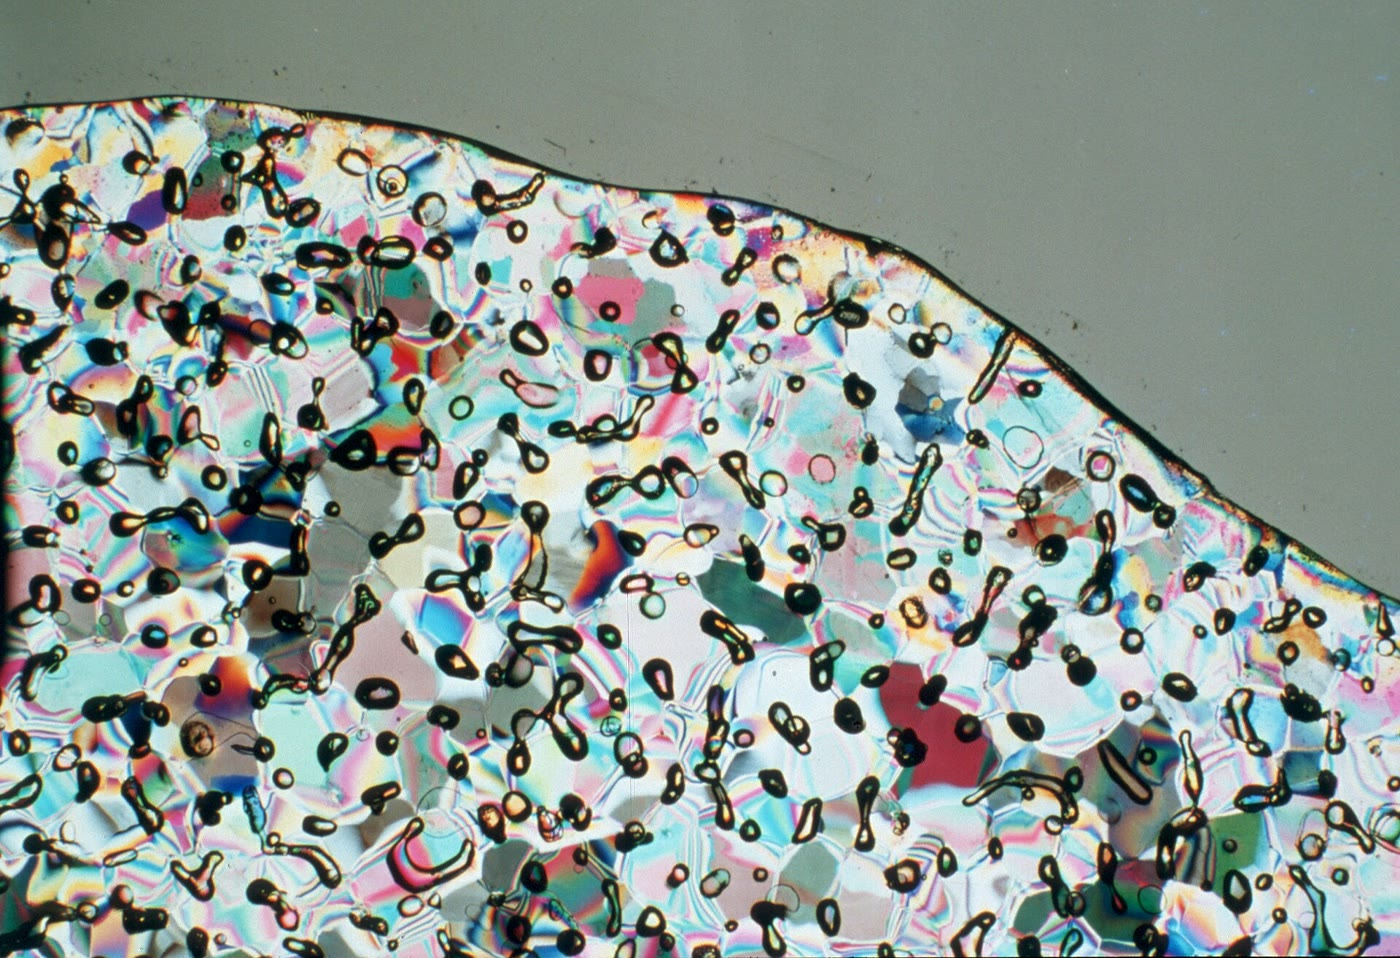
\includegraphics[width=0.50\linewidth]{images/book2/g12-ice-bubbles.jpg}

{\small Selembar tipis es Antarktika yang dilihat di bawah cahaya terpolarisasi,
yang mewarnai kristal-kristal es: titik-titik gelap adalah gelembung udara yang
terperangkap. Foto CSIRO Atmospheric Research, CC~BY~3.0 (Wikimedia Commons).}
\end{omfigure}
% ledger: photo:g12-ice-bubbles

Deuterium inti Dome~C telah diubah menjadi suhu di atas es, yang dinyatakan
sebagai perubahan dibandingkan dengan rata-rata seribu tahun terakhir. Karbon
dioksidanya berasal dari gelembung beberapa inti Antarktika, yang digabungkan
menjadi satu rekaman. Keduanya digambarkan di bawah pada satu sumbu waktu.

\begin{omfigure}
\begin{tikzpicture}
\begin{axis}[omrecord, scale only axis, width=0.74\linewidth, height=4.8cm,
  xmin=0, xmax=800, x dir=reverse, ymin=-12, ymax=8, axis y line*=left,
  xtick={0,100,...,800}, ytick={-10,-5,0,5},
  xlabel={ribuan tahun sebelum 1950},
  ylabel={perubahan suhu (\unit{\degreeCelsius})}]
% data:edc-jouzel, 2-kyr means (figdata/grade-12/ice_age_records.py)
\addplot[omWarm, line width=0.7pt] table[x=age_kyr, y=temp_C] {figdata/out/grade-12-ice_age_records-edc.dat};
\end{axis}
\begin{axis}[scale only axis, width=0.74\linewidth, height=4.8cm,
  xmin=0, xmax=800, x dir=reverse, ymin=60, ymax=320, axis y line*=right,
  axis x line=none, ytick={180,220,260,300}, ylabel={karbon dioksida (ppm)},
  every axis label/.append style={font=\small}, tick label style={font=\small}]
% data:co2-bereiter, 2-kyr means
\addplot[black, line width=0.7pt] table[x=age_kyr, y=co2_ppm] {figdata/out/grade-12-ice_age_records-co2.dat};
\coordinate (lt) at (axis cs:560,70);
\coordinate (lc) at (axis cs:560,312);
\end{axis}
\node[font=\scriptsize, text=omWarm, anchor=south] at (lt) {suhu di Dome~C (skala kiri)};
\node[font=\scriptsize, anchor=north] at (lc) {karbon dioksida (skala kanan)};
\end{tikzpicture}

{\small Delapan ratus ribu tahun es Antarktika, dirata-ratakan dalam langkah
\num{2000} tahun. Merah: suhu di Dome~C dibandingkan dengan seribu tahun
terakhir (Jouzel dan kawan-kawan, 2007); hitam: karbon dioksida dalam gelembung
(Bereiter dan kawan-kawan, 2015). Masa kini ada di sebelah kanan.}
\end{omfigure}
% ledger: data:edc-jouzel, data:co2-bereiter

Kedua kurva itu mempunyai satu pola yang sama: luncuran yang lambat dan
tersendat ke arah dingin selama puluhan ribu tahun, lalu pendakian yang cepat
kembali ke kehangatan, lalu luncuran lagi.

\begin{definition}[Periode glasial; interglasial; siklus glasial]\label{def:g12:past-climates:glacial-cycle}
Yang disebut \emph{periode glasial}\index{periode glasial} adalah selang dingin
dalam sebuah zaman es, ketika lapisan es tumbuh jauh melampaui ukurannya
sekarang. Yang disebut \emph{interglasial}\index{interglasial} adalah selang
hangat di antara dua periode glasial, dengan lapisan es yang mendekati ukuran
sekarang atau lebih kecil; kita hidup dalam salah satunya, yang dimulai sekitar
\num{11000} tahun yang lalu. Yang disebut \emph{siklus
glasial}\index{siklus glasial} adalah satu periode glasial bersama interglasial
yang mengakhirinya.
\end{definition}
% ledger: ipcc:ref-periods (LDT ends 11 ka); the count of cycles is read from the figure (data:edc-jouzel)

Di sepanjang rekaman, suhu di Dome~C berkisar dari
\qty{-10.6}{\degreeCelsius}, sekitar \num{24000} tahun yang lalu, sampai
\qty{+5.5}{\degreeCelsius}, sekitar \num{129000} tahun yang lalu; karbon
dioksidanya, dari \qty{174}{ppm} sampai \qty{299}{ppm}. Gambar itu, yang
dirata-ratakan dalam \num{2000} tahun, sedikit menghaluskan nilai-nilai ekstrem
ini. Hitungan puncak-puncak hangat memberikan delapan atau sembilan \omterm{def:g12:past-climates:glacial-cycle}{siklus
glasial}, dan irama terkuat rekaman suhu itu, yang dihitung dari datanya,
mempunyai periode sekitar \num{98000} tahun.
% ledger: data:edc-jouzel, data:co2-bereiter (ice_age_records.py: edc_min_C -10.58 at 24.0 kyr, edc_max_C 5.46 at 128.7 kyr, co2 173.71 and 298.6, edc_period_kyr 97.5)

\begin{proposition}[Suhu dan karbon dioksida berubah bersama]\label{prop:g12:past-climates:correlation}
% ledger: data:edc-jouzel, data:co2-bereiter (ice_age_records.py: r_temp_co2 0.9165, fit 266.57 + 7.827 T, 1639 pairs)
Selama \num{800000} tahun terakhir, suhu Antarktika dan karbon dioksida udara
berubah bersama. Memasangkan setiap pengukuran dari 1639 pengukuran karbon
dioksida yang lebih tua dari \num{2000} tahun dengan suhu Dome~C pada umur yang
sama memberikan koefisien korelasi $r = 0.92$, dan garis kuadrat terkecil
\[
  \mathrm{CO_2} \approx \qty{267}{ppm} + \qty{7.8}{ppm/\degreeCelsius} \times \Delta T ,
\]
dengan $\Delta T$ perubahan suhu di Dome~C.
\end{proposition}

\begin{proof}[Cara menghitungnya]
Untuk setiap sampel karbon dioksida, suhu pada umurnya dibaca dalam rekaman
Dome~C dengan menginterpolasi antara dua titik suhu yang terdekat. Koefisien
korelasi 1639 pasangan itu, sebuah bilangan antara $-1$ dan $1$ yang mengukur
seberapa dekat titik-titik itu terletak pada sebuah garis lurus (buku-buku
matematika), dihitung bersama garis kuadrat terkecil; keduanya dihitung dalam
skrip gambar dan diperiksa oleh ujinya.
\end{proof}

\begin{omfigure}
\begin{tikzpicture}
\begin{axis}[omrecord, width=0.70\linewidth, height=5.2cm, xmin=-12, xmax=6,
  ymin=160, ymax=310, xlabel={perubahan suhu di Dome~C (\unit{\degreeCelsius})},
  ylabel={karbon dioksida (ppm)}]
% data:edc-jouzel, data:co2-bereiter (pairs and fit in ice_age_records.py)
\addplot[only marks, mark=*, mark size=0.6pt, omDef, opacity=0.45] table[x=temp_C, y=co2_ppm] {figdata/out/grade-12-ice_age_records-pairs.dat};
\addplot[omThm, line width=1pt] table[x=temp_C, y=co2_ppm] {figdata/out/grade-12-ice_age_records-fit.dat};
\node[font=\scriptsize, text=omThm, anchor=south east, fill=white, inner sep=1pt] at (axis cs:-1.5,295) {garis kuadrat terkecil, $r = 0.92$};
\end{axis}
\end{tikzpicture}

{\small Setiap titik adalah satu pengukuran karbon dioksida dalam es Antarktika,
yang ditempatkan pada suhu Dome~C pada umur yang sama: masa-masa dingin
mempunyai sedikit karbon dioksida, masa-masa hangat jauh lebih banyak. Dihitung
dari Jouzel dan kawan-kawan (2007) dan Bereiter dan kawan-kawan (2015).}
\end{omfigure}

Korelasi tidak mengatakan mana yang berubah lebih dahulu, atau apakah ada
penyebab ketiga yang menggerakkan keduanya: koefisiennya akan sama saja bila
suhu menggerakkan karbon dioksida, bila karbon dioksida menggerakkan suhu, atau
bila masing-masing mendorong yang lain. Apa yang menetapkan irama sekitar
\num{100000} tahun itu diceritakan dalam subbab tentang samudra di bawah, dan
bagaimana karbon dioksida bekerja terhadap suhu dalam
\cref{ch:g12:climate-change}.

\subsection{Maksimum Glasial Terakhir}

\begin{definition}[Maksimum Glasial Terakhir]\label{def:g12:past-climates:lgm}
Yang disebut \emph{Maksimum Glasial Terakhir}\index{Maksimum Glasial Terakhir}
adalah masa, sekitar \num{23000} sampai \num{19000} tahun yang lalu, ketika
lapisan es \omterm{def:g12:past-climates:glacial-cycle}{periode glasial} terakhir mencapai ukuran terbesarnya.
\end{definition}
% ledger: ipcc:ref-periods

Pada \omterm{def:g12:past-climates:lgm}{Maksimum Glasial Terakhir}, lapisan es menutupi sebagian besar Amerika Utara
dan Eurasia barat laut, dan iklimnya lebih kering dan lebih berdebu daripada
sekarang. Penilaian-penilaian memperkirakan bahwa suhu permukaan global
\qty{5}{\degreeCelsius} sampai \qty{7}{\degreeCelsius} lebih rendah daripada
pada 1850--1900 (\emph{keyakinan sedang}), dengan karbon dioksida 188 sampai
\qty{194}{ppm}. Air yang terkunci di dalam lapisan es berasal dari samudra:
permukaan laut rata-rata global berada 125 sampai \qty{134}{m} di bawah
permukaan laut sekarang.
% ledger: ipcc:ref-periods, ipcc:lgm-cooling, ipcc:fig2-34, ipcc:lgm-sea, lambeck14:lgm

Laut yang lebih rendah menyingkapkan dasar yang dangkal di sekeliling benua.
Peta di bawah menurunkan permukaan laut \qty{130}{m}, nilai tengah rentang itu,
di atas dasar laut Asia Tenggara seperti keadaannya sekarang.

\begin{omfigure}
\begin{tikzpicture}
\begin{axis}[omrecord, axis equal image, width=0.62\linewidth, xmin=92, xmax=122,
  ymin=-11, ymax=24, grid=none, axis x line=box, axis y line=box,
  xtick={95,105,115}, ytick={-10,-5,...,20},
  xticklabel={\pgfmathprintnumber{\tick}\textdegree BT},
  yticklabels={10\textdegree LS, 5\textdegree LS, 0\textdegree, 5\textdegree LU, 10\textdegree LU, 15\textdegree LU, 20\textdegree LU}]
% data:b2-etopo-sunda (raster computed in ice_age_records.py; sea level lowered by 130 m)
\addplot graphics[xmin=91.95, xmax=122.05, ymin=-11.05, ymax=24.05] {figdata/out/grade-12-ice_age_records-sunda.png};
\node[font=\scriptsize] at (axis cs:114.5,0.5) {Kalimantan};
\node[font=\scriptsize, rotate=-45] at (axis cs:101.9,-1.3) {Sumatra};
\node[font=\scriptsize] at (axis cs:110.5,-8.6) {Jawa};
\node[font=\scriptsize, rotate=-60] at (axis cs:102.2,4.0) {Smj. Malaya};
\node[font=\scriptsize] at (axis cs:103,16.5) {Indocina};
\node[font=\scriptsize, align=center] at (axis cs:106.5,3.5) {Paparan\\Sunda};
\node[font=\scriptsize, align=center] at (axis cs:114.5,13) {Laut Cina\\Selatan};
\node[font=\scriptsize, align=center] at (axis cs:96,-6) {Samudra\\Hindia};
\end{axis}
\end{tikzpicture}

{\small Asia Tenggara dengan permukaan laut \qty{130}{m} lebih rendah daripada
sekarang. Hijau: daratan sekarang; cokelat muda: dasar laut yang tersingkap oleh
permukaan laut yang \qty{130}{m} lebih rendah; biru: laut. Relief sekarang yang
dipakai, sehingga garis pantainya hanya perkiraan. Dihitung dari relief ETOPO1
(NOAA), setiap 0.1 derajat.}
\end{omfigure}
% ledger: data:b2-etopo-sunda, ipcc:lgm-sea

Kalimantan, Sumatra, dan Jawa menyatu dengan Semenanjung Malaya dan Indocina
menjadi satu daratan: Paparan Sunda, yang kini berada di bawah laut dangkal,
dahulu merupakan daratan kering. Pada peta itu, penurunan hanya sekitar
\qty{36}{m} sudah cukup untuk menyatukan Kalimantan dengan Asia, dan Sumatra
dan Jawa menyatu lebih awal lagi. Pada peta itu,
daratan di atas permukaan laut bertambah dari 4.11 menjadi 7.16 juta kilometer
persegi, 1.74 kali lipat. Di seluruh Bumi, penurunan \qty{130}{m} yang sama
menaikkan bagian permukaan yang berada di atas laut dari \qty{29.0}{\percent}
menjadi \qty{33.5}{\percent}, sekitar 23 juta kilometer persegi daratan baru.
% ledger: data:b2-etopo-sunda, data:etopo1 (ice_age_records.py: borneo_link_m -36; sunda_land_now_km2 4.105e6, lgm 7.161e6, ratio 1.744; world_land_now_frac 0.2904, lgm 0.3352, world_gain_km2 2.285e7)

\begin{example}[Deglasiasi terakhir]
Pemanasan yang menyusul \omterm{def:g12:past-climates:lgm}{Maksimum Glasial Terakhir} disebut transisi deglasial
terakhir; penilaian-penilaian menempatkannya antara sekitar \num{18000} dan
\num{11000} tahun yang lalu. Dalam rekaman Dome~C, suhu rata-rata \omterm{def:g12:past-climates:lgm}{Maksimum
Glasial Terakhir} (\num{23000} sampai \num{19000} tahun yang lalu) adalah
\qty{-9.4}{\degreeCelsius}; rata-rata selang berikutnya, \num{11000} sampai
\num{9000} tahun yang lalu, adalah \qty{-0.4}{\degreeCelsius}. Udara di atas
Antarktika menghangat \qty{9.0}{\degreeCelsius}, sementara karbon dioksidanya
naik dari \qty{190}{ppm} menjadi \qty{264}{ppm}, sebesar \qty{74}{ppm}. Di
seluruh Bumi, pemanasannya adalah pendinginan hasil penilaian, 5 sampai
\qty{7}{\degreeCelsius}, sekitar \qty{6}{\degreeCelsius}, yang tersebar selama
\num{7000} tahun transisi itu:
\[
  \frac{\qty{6}{\degreeCelsius}}{\num{7000}\ \text{tahun}} \approx
  \qty{0.86}{\degreeCelsius} \text{ per seribu tahun.}
\]
Sementara itu permukaan laut naik dari sekitar \qty{-120}{m} menjadi
\qty{-50}{m}, rata-rata sekitar \qty{10}{mm} setahun.
\end{example}
% ledger: ipcc:ref-periods, ipcc:lgm-cooling, ipcc:lgm-sea, data:edc-jouzel, data:co2-bereiter (ice_age_records.py: edc_lgm_C -9.389, edc_holo_C -0.360, rise 9.029; co2 189.67, 264.10, rise 74.43; ldt_mean_rate 0.857)

\begin{omfigure}
\begin{tikzpicture}
\begin{axis}[omrecord, scale only axis, width=0.74\linewidth, height=4.6cm,
  xmin=0, xmax=30, x dir=reverse, ymin=-11, ymax=12, axis y line*=left,
  xtick={0,5,...,30}, ytick={-10,-5,0},
  xlabel={ribuan tahun sebelum 1950},
  ylabel={perubahan suhu (\unit{\degreeCelsius})}]
\fill[omDef!10] (axis cs:23,-11) rectangle (axis cs:19,12);
\fill[omProp!12] (axis cs:18,-11) rectangle (axis cs:11,12);
% data:edc-jouzel, every sample
\addplot[omWarm, line width=0.6pt] table[x=age_kyr, y=temp_C] {figdata/out/grade-12-ice_age_records-edc30.dat};
\coordinate (lgm) at (axis cs:21,11.6);
\coordinate (ldt) at (axis cs:14.5,11.6);
\coordinate (lt) at (axis cs:5.5,-3.6);
\end{axis}
\begin{axis}[scale only axis, width=0.74\linewidth, height=4.6cm,
  xmin=0, xmax=30, x dir=reverse, ymin=60, ymax=290, axis y line*=right,
  axis x line=none, ytick={200,240,280}, ylabel={karbon dioksida (ppm)},
  every axis label/.append style={font=\small}, tick label style={font=\small}]
% data:co2-bereiter, every sample
\addplot[black, line width=0.6pt, mark=*, mark size=0.5pt] table[x=age_kyr, y=co2_ppm] {figdata/out/grade-12-ice_age_records-co230.dat};
\coordinate (lc) at (axis cs:26.5,196);
\end{axis}
\node[font=\scriptsize, anchor=north, align=center] at (lgm) {Maksimum\\Glasial Terakhir};
\node[font=\scriptsize, anchor=north, align=center] at (ldt) {transisi deglasial\\terakhir};
\node[font=\scriptsize, text=omWarm, anchor=north] at (lt) {suhu (kiri)};
\node[font=\scriptsize, anchor=south] at (lc) {karbon dioksida (kanan)};
\end{tikzpicture}

{\small \num{30000} tahun terakhir di Dome~C, setiap pengukuran: suhu (merah)
dan karbon dioksida (hitam) naik bersama keluar dari \omterm{def:g12:past-climates:lgm}{Maksimum Glasial Terakhir}.
Diarsir: \omterm{def:g12:past-climates:lgm}{Maksimum Glasial Terakhir} dan transisi deglasial terakhir seperti yang
ditanggali IPCC. Data: Jouzel dan kawan-kawan (2007), Bereiter dan kawan-kawan
(2015).}
\end{omfigure}
% ledger: data:edc-jouzel, data:co2-bereiter, ipcc:ref-periods

\section{Polen}

Setiap musim semi, tumbuhan melepaskan awan polen. Sebagian besar hilang,
tetapi sebagian jatuh di danau dan rawa, tenggelam, dan terkubur di dalam
lumpur, tempat polen itu menyimpan rekaman vegetasi yang tumbuh di sekitarnya.
Dan butir-butir setiap jenis tumbuhan mempunyai bentuk dan ukurannya sendiri.
% ledger: ncei:pollen

\begin{omfigure}
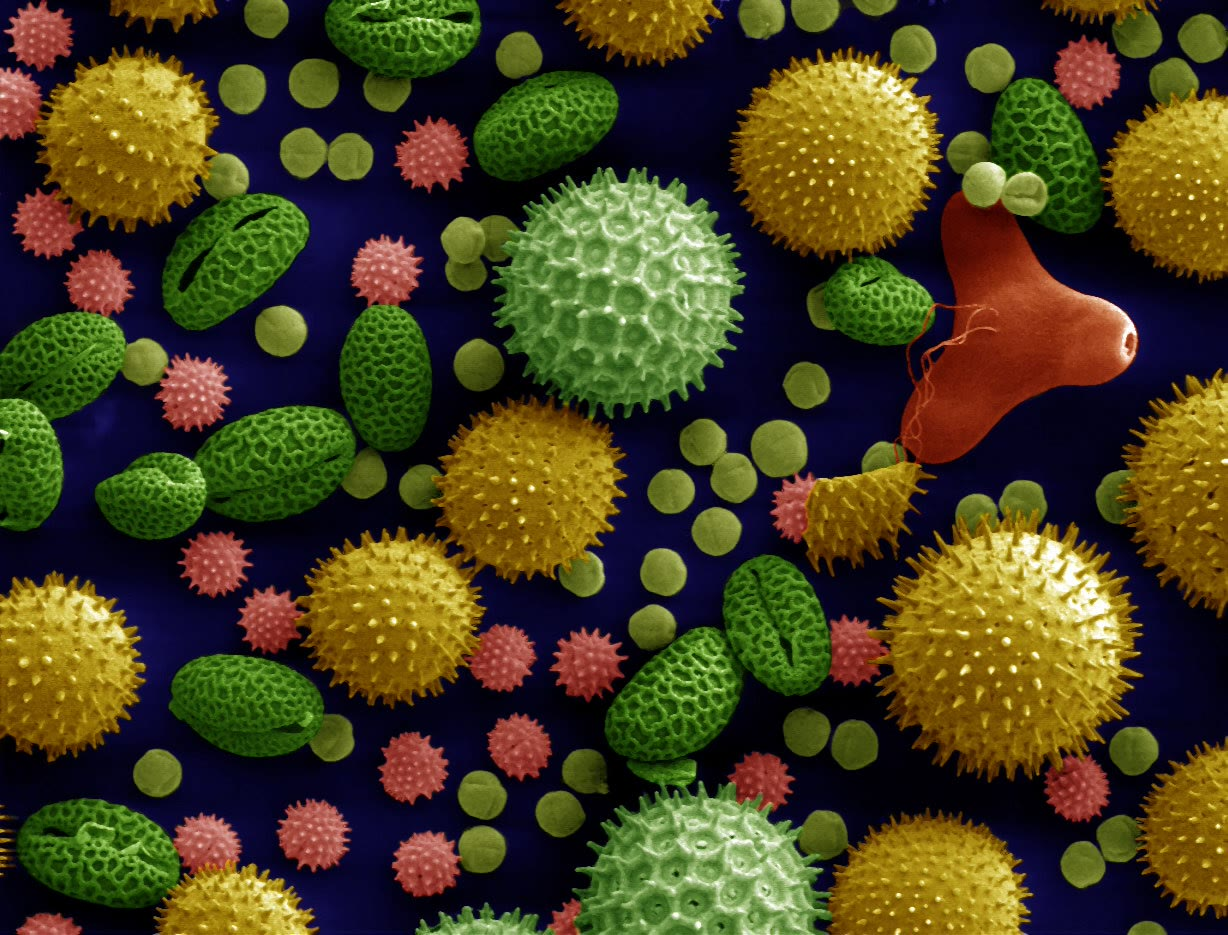
\includegraphics[width=0.46\linewidth]{images/book2/g12-pollen-sem.jpg}

{\small Butir-butir polen lima tumbuhan yang umum (bunga matahari, kangkung
pagar, bunga hollyhock, lili, dan primula) yang dilihat dengan mikroskop elektron
payar, dalam warna palsu. Setiap jenis tumbuhan mempunyai bentuk butirnya
sendiri. Dartmouth Electron Microscope Facility (domain publik, melalui
Wikimedia Commons).}
\end{omfigure}
% ledger: photo:g12-pollen

\begin{definition}[Analisis polen]\label{def:g12:past-climates:pollen}
Yang disebut \emph{analisis polen}\index{analisis polen} adalah pembacaan
vegetasi masa lalu dari polen yang terawetkan dalam sedimen: di setiap lapisan
sebuah inti, butir-butirnya dikenali dan dihitung, dan bagian setiap jenis
tumbuhan, dalam persen dari butir yang dihitung, diplot terhadap kedalaman dalam
sebuah \emph{diagram polen}\index{diagram polen}.
\end{definition}
% ledger: ncei:pollen

Penghitungan polen dengan cara ini dimulai oleh ahli geologi Swedia Lennart von
Post, yang menyajikan \omterm{def:g12:past-climates:pollen}{diagram polen} modern pertama, dengan angka-angka, pada
tahun 1916; diagram seperti itu menunjukkan kedalaman ke arah bawah halaman dan
satu kurva untuk setiap jenis tumbuhan. Vegetasi, pada gilirannya, berbicara
tentang iklim: rumput dan herba lain yang hampir tanpa pohon berarti bentang
alam yang terbuka dan dingin, sedangkan ek dan hazel memerlukan musim panas
yang hangat.
% ledger: rull18:von-post; the Varden diagram is invented (ice_age_records.py POLLEN)

\begin{omfigure}
\begin{tikzpicture}
\pgfplotsset{pollen/.style={scale only axis, height=6cm, ymin=300, ymax=600,
  y dir=reverse, xmin=0, axis x line*=bottom, axis y line*=left, axis line style={-},
  tick label style={font=\scriptsize}, title style={font=\small, yshift=-4pt, text depth=0.25ex, text height=1.6ex},
  ytick={300,350,...,600}, xmajorgrids, ymajorgrids,
  grid style={gray!22, line width=0.3pt}}}
\begin{axis}[pollen, name=p1, width=3.0cm, xmax=100, xtick={0,20,...,80}, title={herba},
  ylabel={kedalaman (cm)}, every axis label/.append style={font=\small}]
\addplot[fill=omLithSand, draw=black!70, line width=0.4pt] table[x=pct, y=depth_cm] {figdata/out/grade-12-ice_age_records-pol-herbs.dat};
\coordinate (z1) at (axis cs:0,550);
\coordinate (z2) at (axis cs:0,470);
\coordinate (z3) at (axis cs:0,425);
\end{axis}
\begin{axis}[pollen, name=p2, at={(p1.south east)}, anchor=south west, xshift=0.3cm,
  width=1.8cm, xmax=60, xtick={0,20,40}, title={birch}, yticklabels={}]
\addplot[fill=omHypsLandB, draw=black!70, line width=0.4pt] table[x=pct, y=depth_cm] {figdata/out/grade-12-ice_age_records-pol-birch.dat};
\end{axis}
\begin{axis}[pollen, name=p3, at={(p2.south east)}, anchor=south west, xshift=0.3cm,
  width=1.8cm, xmax=60, xtick={0,20,40}, title={pinus}, yticklabels={}]
\addplot[fill=omHypsLandA, draw=black!70, line width=0.4pt] table[x=pct, y=depth_cm] {figdata/out/grade-12-ice_age_records-pol-pine.dat};
\end{axis}
\begin{axis}[pollen, name=p4, at={(p3.south east)}, anchor=south west, xshift=0.3cm,
  width=1.2cm, xmax=40, xtick={0,20}, title={hazel}, yticklabels={}]
\addplot[fill=omHypsLandD, draw=black!70, line width=0.4pt] table[x=pct, y=depth_cm] {figdata/out/grade-12-ice_age_records-pol-hazel.dat};
\end{axis}
\begin{axis}[pollen, name=p5, at={(p4.south east)}, anchor=south west, xshift=0.3cm,
  width=1.5cm, xmax=50, xtick={0,20,40}, title={ek}, yticklabels={}]
\addplot[fill=omHypsLandE, draw=black!70, line width=0.4pt] table[x=pct, y=depth_cm] {figdata/out/grade-12-ice_age_records-pol-oak.dat};
\coordinate (e1) at (axis cs:50,550);
\coordinate (e2) at (axis cs:50,470);
\coordinate (e3) at (axis cs:50,425);
\coordinate (top) at (axis cs:50,300);
\coordinate (bot) at (axis cs:50,600);
\end{axis}
\draw[densely dashed, black!70] (z1) -- (e1 -| p5.east);
\draw[densely dashed, black!70] (z2) -- (e2 -| p5.east);
\draw[densely dashed, black!70] (z3) -- (e3 -| p5.east);
\node[font=\scriptsize, anchor=west] at ($(bot -| p5.east)!0.5!(e1 -| p5.east)$) {zona 1};
\node[font=\scriptsize, anchor=west] at ($(e1 -| p5.east)!0.5!(e2 -| p5.east)$) {zona 2};
\node[font=\scriptsize, anchor=west] at ($(e2 -| p5.east)!0.5!(e3 -| p5.east)$) {zona 3};
\node[font=\scriptsize, anchor=west] at ($(e3 -| p5.east)!0.5!(top -| p5.east)$) {zona 4};
\node[font=\scriptsize, anchor=north] at ($(p1.south)!0.5!(p5.south)+(0,-0.45)$) {persen dari polen yang dihitung};
\end{tikzpicture}

{\small \omterm{def:g12:past-climates:pollen}{Diagram polen} sebuah danau di Perbukitan Varden, wilayah rekaan seri
ini: data latihan rekaan, dengan suksesi yang dijumpai di banyak danau di zona
sedang yang sejuk. Dasar inti (\qty{600}{cm}) berumur \num{14000} tahun,
puncak yang ditampilkan (\qty{300}{cm}) \num{6000} tahun, dengan laju
pengendapan yang tetap di antaranya.}
\end{omfigure}
% invented exercise data (ice_age_records.py POLLEN); no ledger row

\begin{method}[Membaca diagram polen]
\begin{enumerate}
  \item Bacalah sumbu tegaknya: kedalaman, lapisan tertua di bawah; ubahlah
        kedalaman menjadi umur dengan tanggal-tanggal inti itu.
  \item Untuk setiap lapisan, temukan tumbuhan dengan bagian terbesar.
  \item Bagilah inti itu menjadi zona-zona, masing-masing dengan kelompok
        tumbuhan dominannya sendiri; letakkan batas-batasnya di tempat
        kurva-kurva berubah paling cepat.
  \item Namailah vegetasi setiap zona (herba terbuka, hutan birch, hutan
        pinus, hutan daun lebar) dan iklim yang diperlukannya.
  \item Bacalah zona-zona itu dari bawah ke atas sebagai sejarah bentang
        alam.
\end{enumerate}
\end{method}

Dalam diagram di atas, zona 1 adalah bentang alam herba, dengan sedikit birch:
daerah terbuka dan dingin yang ditinggalkan es. Di zona 2, birch menyebar lebih
dahulu, sebuah pohon yang tahan; pinus menyusul di zona 3; dan di zona 4 hazel
dan ek, yang memerlukan musim panas yang hangat, mengambil alih. Dibaca dari
bawah ke atas, inti itu menceritakan berakhirnya \omterm{def:g12:past-climates:glacial-cycle}{periode glasial} dan datangnya
kehangatan \omterm{def:g12:past-climates:glacial-cycle}{interglasial}, ketika hutan kembali menyebar ke daratan.

\section{Sedimen samudra dan irama astronomis}

Di dasar samudra terbuka, lumpur menumpuk perlahan dan tanpa putus, lapis demi
lapis, selama jutaan tahun. Lumpur itu penuh dengan cangkang foraminifera:
organisme bersel tunggal yang cangkangnya, berukuran sepecahan milimeter,
sering terbuat dari kalsit. Sebagian melayang di dekat permukaan; yang lain
hidup di dasar laut.
% ledger: ucmp:forams, lr04:stack (benthic), photo:g12-forams (planktic)

\begin{omfigure}
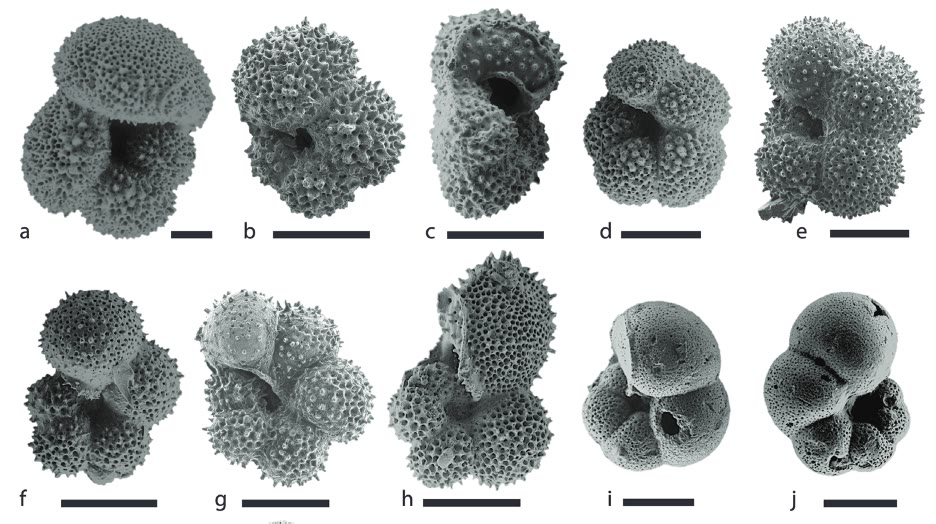
\includegraphics[width=0.62\linewidth]{images/book2/g12-planktic-foraminifera.jpg}

{\small Cangkang sepuluh spesies foraminifera yang hidup melayang di samudra,
dilihat dengan mikroskop elektron payar; setiap batang skala berukuran
\qty{150}{\micro\metre}, sehingga setiap cangkang kira-kira sebesar sebutir
pasir. Marci Robinson, USGS (domain publik, melalui Wikimedia Commons).}
\end{omfigure}
% ledger: photo:g12-forams

Oksigen sebuah cangkang berasal dari air laut. Air yang tersusun dari isotop
ringan oksigen-16 lebih mudah menguap, dan karena itu salju yang membangun
lapisan es miskin oksigen-18. Ketika lapisan es tumbuh, lapisan es menyimpan
air ringan ini, dan samudra yang tertinggal menjadi lebih kaya oksigen-18;
demikian pula cangkang-cangkang yang tumbuh di dalamnya, terlebih lagi bila
airnya lebih dingin. Bagian oksigen-18 dalam cangkang foraminifera dasar laut,
yang ditulis $\delta^{18}\mathrm{O}$ dan dinyatakan dalam bagian per seribu,
dengan demikian merupakan \omterm{def:g12:past-climates:proxy}{proksi} volume es di daratan dan suhu \omterm{def:g10:layered-ocean:thermocline}{samudra dalam}:
makin tinggi nilainya, makin banyak es dan makin dingin airnya.
% ledger: nasaeo:o18, lr04:stack

Rekaman di bawah, yang disebut LR04, menumpuk pengukuran 57 inti dari semua
samudra menjadi satu kurva sepanjang 5.3 juta tahun.

\begin{omfigure}
\begin{tikzpicture}
\begin{axis}[omrecord, scale only axis, width=0.86\linewidth, height=4.8cm,
  xmin=0, xmax=5.32, x dir=reverse, ymin=2.4, ymax=5.3, y dir=reverse,
  xtick={0,0.5,...,5}, ytick={2.5,3,...,5},
  x tick label style={/pgf/number format/.cd, fixed, precision=1},
  y tick label style={/pgf/number format/.cd, fixed, fixed zerofill, precision=1},
  xlabel={jutaan tahun sebelum 1950},
  ylabel={$\delta^{18}\mathrm{O}$ cangkang (\unit{\permil})}]
\fill[omProp!14] (axis cs:1.25,2.4) rectangle (axis cs:0.7,5.3);
% data:lr04 (the stack only; ice_age_records.py)
\addplot[omDef!85!black, line width=0.35pt] table[x=age_Ma, y=d18O] {figdata/out/grade-12-ice_age_records-lr04.dat};
\addplot[omThm, line width=1pt, densely dashed, unbounded coords=jump] table[x=age_Ma, y=d18O] {figdata/out/grade-12-ice_age_records-lr04mean.dat};
\coordinate (mpt) at (axis cs:0.975,2.45);
\coordinate (mm) at (axis cs:5.22,4.92);
\coordinate (arr) at (axis cs:5.12,3.9);
\end{axis}
\node[font=\scriptsize, anchor=north, align=center] at (mpt) {41 000 sampai\\100 000 tahun};
\draw[omThm, line width=1pt, densely dashed] (mm) -- ($(mm)+(0.5,0)$) node[right, font=\scriptsize, text=omThm] {rata-rata 5.3 sampai 3 dan 1 sampai 0 juta tahun yang lalu};
\draw[-{Stealth}, black!70] (arr) -- ++(0,-0.9) node[midway, right, font=\scriptsize, align=left] {lebih banyak es,\\lebih dingin};
\end{tikzpicture}

{\small Lima juta tahun \omterm{def:g10:layered-ocean:thermocline}{samudra dalam} di dalam cangkang foraminifera dasar laut;
sumbu tegaknya dibalik, sehingga masa-masa yang dingin dan penuh es berada di
bawah. Garis putus-putus adalah rata-rata bagian pertama dan terakhir. Diarsir:
peralihan dari irama \num{41000} tahun ke irama sekitar \num{100000} tahun.
Data: Lisiecki dan Raymo (2005), tumpukan LR04.}
\end{omfigure}
% ledger: data:lr04, lr04:stack, clark06:mpt

Dibaca dengan metode di atas, rekaman itu mengatakan tiga hal.
\begin{itemize}
  \item \emph{Bumi telah mendingin dan esnya telah bertambah.} Nilai
        rata-ratanya naik dari \qty{3.03}{\permil} antara 5.3 dan 3 juta tahun
        yang lalu menjadi \qty{4.15}{\permil} selama sejuta tahun terakhir.
  \item \emph{Ayunannya telah membesar.} Masa glasial dan \omterm{def:g12:past-climates:glacial-cycle}{interglasial}
        bergantian di sepanjang rekaman, tetapi ayunannya makin lebar: pada
        \omterm{def:g12:past-climates:lgm}{Maksimum Glasial Terakhir} nilainya \qty{4.92}{\permil}, dibandingkan
        dengan \qty{3.23}{\permil} sekarang.
  \item \emph{Iramanya telah berubah.} Antara 2.6 dan 1.3 juta tahun yang
        lalu, periode terkuat rekaman itu, yang dihitung dari datanya, adalah
        \num{41000} tahun; selama \num{700000} tahun terakhir periode itu sekitar
        \num{98000} tahun, irama \omterm{def:g12:past-climates:ice-core}{inti es}. Perubahan itu terjadi antara sekitar
        1.25 dan 0.7 juta tahun yang lalu.
\end{itemize}
% ledger: data:lr04, clark06:mpt (ice_age_records.py: lr04_mean_3_5Ma 3.032, lr04_mean_0_1Ma 4.147, lr04_lgm 4.92, lr04_today 3.23, periods 41.0 and 98.5 kyr)

Periode-periode ini bukan kebetulan. Pada tahun 1976, James Hays, John Imbrie,
dan Nicholas Shackleton menemukan dalam sedimen samudra selatan tiga irama,
\num{23000}, \num{42000}, dan sekitar \num{100000} tahun, yang merupakan
periode perubahan lambat orbit dan sumbu Bumi: presesi sumbu, kemiringan sumbu
(sekitar \num{41000} tahun), dan bentuk orbit (sekitar \num{100000} tahun).
Perubahan-perubahan ini menggeser sinar Matahari yang diterima setiap lintang
pada setiap musim, dan perubahan itu menetapkan tempo siklus-siklus glasial.
Bagaimana hal itu terjadi, dan mengapa irama lambat \num{100000} tahun
mengambil alih, adalah pokok bahasan kuliah di universitas.
% ledger: hays76:periods, nasa:milankovitch, lr04:stack, clark06:mpt

\begin{dated}{2025}
Pada Januari 2025, proyek Beyond EPICA mengumumkan bahwa sebuah inti yang dibor
di Little Dome~C, sekitar \qty{35}{km} dari stasiun Concordia di Dome~C,
menyimpan rekaman yang tak terputus sampai sekitar 1.2 juta tahun yang lalu
dalam \qty{2480}{m} bagian atasnya. Rekaman itu meliputi masa
ketika irama glasial berubah dari \num{41000} menjadi \num{100000} tahun, dan
es serta udaranya sedang dianalisis.
\end{dated}
% ledger: ku25:beyond-epica, ipev25:little-dome-c

\section{Iklim masa geologi yang jauh}

Lebih jauh ke belakang daripada \omterm{def:g12:past-climates:ice-core}{inti es}, iklim masa lalu dibaca dari sedimen,
daun dan tanah fosil, serta isotop. IPCC telah memilih beberapa \emph{periode
acuan}, yang telah banyak dikaji, yang iklimnya membantu menilai perubahan masa
kini dan masa depan. Bagan di bawah memberikan suhu permukaan globalnya,
dibandingkan dengan 1850--1900.

\begin{omfigure}
\begin{tikzpicture}
\begin{axis}[omrecord, width=0.86\linewidth, height=5.4cm, xmin=-9, xmax=27,
  ymin=0.4, ymax=6.6, y dir=reverse, ytick={1,...,6}, ymajorgrids=false,
  yticklabels={{PETM, 56 Ma}, {EECO, 53--49 Ma}, {MPWP, 3.3--3.0 Ma},
    {LIG, 129--116 ka}, {LGM, 23--19 ka}, {MH, 6.5--5.5 ka}},
  y tick label style={font=\scriptsize},
  xlabel={suhu dibandingkan dengan 1850--1900 (\unit{\degreeCelsius})}]
% ipcc:fig2-34 (DEEP in ice_age_records.py)
\addplot[draw=none, mark=none, restrict expr to domain={\thisrow{tlo}}{0:30},
  error bars/.cd, x dir=both, x explicit,
  error bar style={line width=5pt, omWarm!75}, error mark=none]
  table[x expr={(\thisrow{tlo}+\thisrow{thi})/2}, y=idx,
        x error expr={(\thisrow{thi}-\thisrow{tlo})/2}] {figdata/out/grade-12-ice_age_records-deep.dat};
\addplot[draw=none, mark=none, restrict expr to domain={\thisrow{tlo}}{-30:-0.01},
  error bars/.cd, x dir=both, x explicit,
  error bar style={line width=5pt, omCold!75}, error mark=none]
  table[x expr={(\thisrow{tlo}+\thisrow{thi})/2}, y=idx,
        x error expr={(\thisrow{thi}-\thisrow{tlo})/2}] {figdata/out/grade-12-ice_age_records-deep.dat};
\draw[black!60] (axis cs:0,0.4) -- (axis cs:0,6.6);
\draw[omThm, densely dashed, line width=0.8pt] (axis cs:1.09,0.4) -- (axis cs:1.09,6.6);
\node[font=\scriptsize, text=omThm, anchor=west, fill=white, inner sep=1pt] at (axis cs:1.6,4.55) {2011--2020};
\end{axis}
\end{tikzpicture}

{\small Suhu permukaan global enam periode acuan masa lalu, rentang
sangat mungkin, dibandingkan dengan 1850--1900; putus-putus: dekade
2011--2020. PETM: Maksimum Termal Paleosen--Eosen; EECO: Optimum Iklim Eosen
Awal; MPWP: Periode Hangat Pliosen tengah; LIG: Interglasial Terakhir; LGM:
\omterm{def:g12:past-climates:lgm}{Maksimum Glasial Terakhir}, satu-satunya yang dingin (biru); MH: Holosen tengah.
Nilai: IPCC AR6 WG1, Gambar 2.34.}
\end{omfigure}
% ledger: ipcc:fig2-34, ipcc:gsat-2011-2020, ipcc:ref-periods

\begin{center}
\small
\begin{tabular}{|l|c|c|c|}
\hline
\textbf{periode} & \textbf{suhu (\unit{\degreeCelsius})} & \textbf{karbon dioksida (ppm)} & \textbf{permukaan laut (m)} \\
\hline
PETM, 56 Ma & $+10$ sampai $+25$ & sekitar 900, naik menjadi 2000 & --- \\
EECO, 53--49 Ma & $+10$ sampai $+18$ & 1150 sampai 2500 & $+70$ sampai $+76$ \\
MPWP, 3.3--3.0 Ma & $+2.5$ sampai $+4.0$ & 360 sampai 420 & $+5$ sampai $+25$ \\
LIG, 129--116 ka & $+0.5$ sampai $+1.5$ & 266 sampai 282 & $+5$ sampai $+10$ \\
\textcolor{omCold}{LGM, 23--19 ka} & \textcolor{omCold}{$-7$ sampai $-5$} & \textcolor{omCold}{188 sampai 194} & \textcolor{omCold}{$-134$ sampai $-125$} \\
MH, 6.5--5.5 ka & $+0.2$ sampai $+1.0$ & 260 sampai 268 & $-3.5$ sampai $+0.5$ \\
\hline
\end{tabular}

\medskip
{\small Periode-periode acuan: suhu permukaan global dibandingkan dengan
1850--1900, karbon dioksida, dan permukaan laut global dibandingkan dengan 1900.
IPCC AR6 WG1, Gambar 2.34.}
\end{center}
% ledger: ipcc:fig2-34

Maksimum Termal Paleosen--Eosen adalah pemanasan yang mendadak, ketika
sejumlah besar karbon secara tiba-tiba mencapai samudra dan udara: samudra
menjadi lebih asam dan lebih miskin oksigen, dan banyak spesies laut dalam
punah. Pada Optimum Iklim Eosen Awal, karbon dioksida tetap di atas
\qty{1000}{ppm} selama jutaan tahun, tidak ada es kutub, dan hutan yang
mendekati hutan tropis tumbuh pada \ang{70} lintang selatan. Periode Hangat
Pliosen tengah adalah masa terakhir ketika karbon dioksida mendekati kadar
sekarang: Arktika jauh lebih hangat daripada sekarang, dan permukaan laut lebih
tinggi. Pada Interglasial Terakhir, lapisan es Greenland dan Antarktika Barat
lebih kecil dan permukaan laut lebih tinggi daripada sekarang, dan kuda nil
hidup di Britania.
% ledger: ipcc:ref-periods, ipcc:fig2-34, ipcc:mpwp-eeco

Arsip-arsip ini menempatkan masa kini dalam perspektif, dan IPCC sendiri
membuat perbandingan itu. Pada tahun 2019 karbon dioksida udara lebih tinggi
daripada kapan pun dalam setidaknya dua juta tahun (\emph{keyakinan tinggi}),
dan kenaikan karbon dioksida dan metana sejak 1750 jauh melampaui perubahan
alami antara \omterm{def:g12:past-climates:glacial-cycle}{periode glasial} dan \omterm{def:g12:past-climates:glacial-cycle}{interglasial} selama setidaknya \num{800000}
tahun (\emph{keyakinan sangat tinggi}). Suhu permukaan global telah naik lebih
cepat sejak 1970 daripada dalam periode 50 tahun lain mana pun selama
setidaknya \num{2000} tahun terakhir (\emph{keyakinan tinggi}). Dekade
2011--2020 lebih hangat daripada abad-abad terhangat \omterm{def:g12:past-climates:glacial-cycle}{interglasial} sekarang,
sekitar \num{6500} tahun yang lalu, dan mendekati kehangatan Interglasial
Terakhir, sekitar \num{125000} tahun yang lalu (\emph{keyakinan sedang}).
% ledger: ipcc:co2-ch4-800kyr, ipcc:fastest-2000yr, ipcc:co2-2myr

Kecepatan perubahan itu juga dapat dibandingkan. Dari 1970 sampai 2025, tren
rekaman suhu global adalah \qty{0.20}{\degreeCelsius} per dekade, atau sekitar
\qty{20}{\degreeCelsius} per seribu tahun bila terus berlanjut; pemanasan
keluar dari \omterm{def:g12:past-climates:glacial-cycle}{periode glasial} terakhir rata-rata sekitar
\qty{0.86}{\degreeCelsius} per seribu tahun. Penyebab perubahan masa kini, dan
akan menjadi apa perubahan itu, adalah pokok bahasan
\cref{ch:g12:climate-change}.
% ledger: data:gistemp (ice_age_records.py: rate_1970_2025_C_per_decade 0.2012), ipcc:lgm-cooling, ipcc:ref-periods

\section{Latihan}

\begin{exercise}[$\star$]\label{exo:g12:past-climates:1}
Sebutkan istilahnya: (a) besaran yang diukur dalam sebuah arsip yang mewakili
suatu variabel iklim yang tidak diukur; (b) silinder es yang dibor dari lapisan
es; (c) selang hangat di antara dua \omterm{def:g12:past-climates:glacial-cycle}{periode glasial}; (d) pembacaan vegetasi
masa lalu dari polen fosil; (e) masa, sekitar \num{23000} sampai \num{19000}
tahun yang lalu, ketika lapisan es terakhir paling besar.
\end{exercise}

\begin{exercise}[$\star$]\label{exo:g12:past-climates:2}
Untuk setiap \omterm{def:g12:past-climates:proxy}{proksi}, sebutkan arsipnya dan apa yang diberitahukannya: (a) udara
dalam gelembung; (b) bagian polen ek; (c) oksigen-18 dalam cangkang
foraminifera dasar laut; (d) lebar lingkaran tahun pohon.
\end{exercise}

\begin{exercise}[$\star$]\label{exo:g12:past-climates:3}
Selama transisi deglasial terakhir, dari sekitar \num{18000} sampai
\num{11000} tahun yang lalu, permukaan laut naik dari sekitar \qty{-120}{m}
menjadi \qty{-50}{m}. (a) Hitung laju kenaikan rata-ratanya, dalam milimeter
per tahun. (b) Dari 2006 sampai 2018, permukaan laut naik \qty{3.7}{mm}
setahun. Bandingkan.
\end{exercise}

\begin{exercise}[$\star$]\label{exo:g12:past-climates:4}
Suhu global naik \qty{0.20}{\degreeCelsius} per dekade dari 1970 sampai 2025.
Nyatakan laju ini per abad dan per seribu tahun.
\end{exercise}

\begin{exercise}[$\star$]\label{exo:g12:past-climates:5}
Hays, Imbrie, dan Shackleton menemukan tiga irama dalam sedimen samudra:
\num{23000}, \num{42000}, dan sekitar \num{100000} tahun. (a) Pasangkan
masing-masing dengan presesi sumbu, kemiringan sumbu, dan bentuk orbit.
(b) Berapa siklus \num{41000} tahun yang muat dalam \num{1000000} tahun? Berapa
siklus \num{100000} tahun?
\end{exercise}

\begin{exercise}[$\star\star$]\label{exo:g12:past-climates:6}
Garis kuadrat terkecil dalam bab ini adalah $\mathrm{CO_2} \approx 266.6 +
7.83\,\Delta T$ (ppm, dengan $\Delta T$ dalam \unit{\degreeCelsius}).
(a) Ramalkan karbon dioksida untuk suhu rata-rata \omterm{def:g12:past-climates:lgm}{Maksimum Glasial Terakhir} di
Dome~C, \qty{-9.4}{\degreeCelsius}, lalu bandingkan dengan \qty{190}{ppm} yang
terukur. (b) Ramalkan untuk titik terhangat, \qty{+5.5}{\degreeCelsius}, lalu
bandingkan dengan nilai terukur tertinggi, \qty{299}{ppm}. (c) Gunakan garis itu
untuk memperkirakan suhu Dome~C yang akan sepadan dengan \qty{427}{ppm}, nilai
tahun 2025 di Mauna Loa. Mengapa penggunaan garis yang terakhir ini tidak
dapat dibenarkan?
\end{exercise}

\begin{exercise}[$\star\star$]\label{exo:g12:past-climates:7}
Gunakan \omterm{def:g12:past-climates:pollen}{diagram polen} danau di Perbukitan Varden. (a) Apa polen yang dominan
pada \qty{580}{cm}, dan bentang alam apa yang ditunjukkannya? (b) Pertanyaan
yang sama pada \qty{340}{cm}. (c) Pohon mana yang menyebar lebih dahulu setelah
masa dingin, dan pohon mana yang datang paling akhir? (d) Mengapa datangnya
sebuah pohon dapat tertinggal di belakang pemanasan yang memungkinkannya?
\end{exercise}

\begin{exercise}[$\star\star$]\label{exo:g12:past-climates:8}
Dalam inti yang sama, lumpur pada \qty{600}{cm} berumur \num{14000} tahun dan
lumpur pada \qty{300}{cm} \num{6000} tahun, dengan laju pengendapan yang tetap.
(a) Hitung laju ini dalam milimeter per tahun. (b) Tentukan umur batas antara
zona 2 dan 3, pada \qty{470}{cm}. (c) Irisan setebal \qty{1}{cm} mewakili
berapa tahun?
\end{exercise}

\begin{exercise}[$\star\star$]\label{exo:g12:past-climates:9}
Pada peta Asia Tenggara, daratan di atas permukaan laut bertambah dari 4.11
menjadi 7.16 juta kilometer persegi bila permukaan laut diturunkan
\qty{130}{m}. (a) Hitung pertambahannya dan persentasenya. (b) Pada peta itu,
penurunan sekitar \qty{36}{m} sudah cukup untuk menyatukan Kalimantan dengan
Asia. Apakah pulau itu menyatu selama seluruh \omterm{def:g12:past-climates:lgm}{Maksimum Glasial Terakhir}?
Jelaskan. (c) Mengapa garis pantai pada peta itu hanya perkiraan?
\end{exercise}

\begin{exercise}[$\star\star$]\label{exo:g12:past-climates:10}
Dalam rekaman LR04, nilai pada \omterm{def:g12:past-climates:lgm}{Maksimum Glasial Terakhir} adalah
\qty{4.92}{\permil} dan nilai sekarang \qty{3.23}{\permil}. (a) Mana yang lebih
tinggi, dan apakah itu yang kamu harapkan? Jelaskan dengan lapisan es.
(b) Mengapa sumbu tegak rekaman itu digambar terbalik?
\end{exercise}

\begin{exercise}[$\star\star$]\label{exo:g12:past-climates:11}
Seorang teman berkata: ``Korelasi 0.92 antara suhu Antarktika dan karbon
dioksida membuktikan bahwa karbon dioksida mengendalikan zaman-zaman es.''
(a) Apa yang ditunjukkan sebuah korelasi, dan apa yang tidak ditunjukkannya?
(b) Berikan dua penjelasan lain yang akan memberikan korelasi yang sama.
(c) Informasi seperti apa tentang kedua rekaman itu yang akan membantu
memutuskannya?
\end{exercise}

\begin{exercise}[$\star\star\star$]\label{exo:g12:past-climates:12}
Periode terkuat rekaman LR04 adalah \num{41000} tahun antara 2.6 dan 1.3 juta
tahun yang lalu, dan \num{98500} tahun selama \num{700000} tahun terakhir.
(a) Berapa siklus yang dimuat setiap jendela itu? (b) Perubahan orbit atau
sumbu Bumi mana yang cocok dengan setiap periode? (c) Jelaskan mengapa rekaman
dengan satu sampel setiap \num{2000} tahun dapat menunjukkan irama-irama ini,
tetapi tidak dapat menunjukkan perubahan yang berlangsung seabad.
\end{exercise}

\begin{exercise}[$\star\star\star$]\label{exo:g12:past-climates:13}
Laju kenaikan karbon dioksida adalah 192 sampai \qty{198}{ppm} per abad pada
1995--2014. Selama Maksimum Termal Paleosen--Eosen laju itu 4 sampai
\qty{42}{ppm} per abad, dan selama transisi deglasial terakhir paling tinggi
sekitar \qty{10}{ppm} per abad. (a) Berapa kali lebih cepat kenaikan baru-baru
ini daripada kenaikan tercepat deglasiasi terakhir? (b) Daripada perkiraan
terlambat dan tercepat PETM? (c) Kenaikan PETM berlangsung dari sekitar 900
sampai sekitar \qty{2000}{ppm}. Berapa lama waktu yang diperlukan dengan laju
\qty{42}{ppm} per abad, dan dengan laju sekarang?
\end{exercise}

\begin{exercise}[$\star\star\star$]\label{exo:g12:past-climates:14}
IPCC memperkirakan bahwa suhu global naik 1 sampai
\qty{1.5}{\degreeCelsius} per seribu tahun pada bagian tercepat deglasiasi
terakhir, dan bahwa di atas Greenland suhu naik sekitar sepuluh kali lebih
cepat pada abad-abad pemanasan yang paling pesat. (a) Berikan laju Greenland
dalam \unit{\degreeCelsius} per seribu tahun dan per dekade. (b) Bandingkan
dengan laju global sekarang, \qty{0.20}{\degreeCelsius} per dekade.
(c) Mengapa laju lokal tidak boleh dibandingkan langsung dengan laju global?
\end{exercise}

\begin{exercise}[$\star\star\star$]\label{exo:g12:past-climates:15}
Permukaan laut sekitar \qty{-50}{m} \num{11000} tahun yang lalu; andaikan
permukaan laut kemudian naik dengan laju tetap \qty{12}{m} per seribu tahun,
laju rata-rata deglasiasi utama. (a) Kapan permukaan laut melewati
\qty{-36}{m}, aras yang menyatukan Kalimantan dengan Asia pada peta itu?
(b) Setelah waktu itu, dapatkah seseorang berjalan kaki dari Kalimantan ke
Semenanjung Malaya? (c) Berapa lama laut akan naik sebesar \qty{36}{m}
terakhir, bila terus berlanjut dengan kecepatan yang sama?
\end{exercise}

\begin{problem}[{Soal akhir pekan --- 800 000 tahun es Antarktika}]
\label{pb:g12:past-climates:1}
% ledger: data:edc-jouzel, data:co2-bereiter, data:lr04, data:gistemp, ipcc:lgm-cooling, ipcc:ref-periods, hays76:periods, clark06:mpt
% values (ice_age_records.py): edc -10.58 / +5.46, co2 173.71 / 298.6, r 0.9165, fit 266.57 + 7.827 T,
% LGM -9.389 / 189.67, 11-9 ka -0.360 / 264.10, period 97.5, rate 0.2012 per decade, ratio 23.48
Es Dome~C dan udara dalam gelembung-gelembungnya memberikan nilai-nilai berikut.
Suhu adalah perubahan di atas es dibandingkan dengan seribu tahun terakhir.

\begin{center}
\small
\begin{tabular}{|l|c|c|}
\hline
 & \textbf{perubahan suhu (\unit{\degreeCelsius})} & \textbf{karbon dioksida (ppm)} \\
\hline
nilai terdingin, sekitar \num{24000} tahun lalu & $-10.6$ & --- \\
nilai terhangat, sekitar \num{129000} tahun lalu & $+5.5$ & --- \\
karbon dioksida terendah dan tertinggi & --- & 174 dan 299 \\
rata-rata, \num{23000} sampai \num{19000} tahun lalu & $-9.4$ & 190 \\
rata-rata, \num{11000} sampai \num{9000} tahun lalu & $-0.4$ & 264 \\
\hline
\end{tabular}
\end{center}

Periode terkuat rekaman suhu itu sekitar \num{98000} tahun, dan 1639 pasang
nilai memberikan koefisien korelasi 0.92.

\medskip
\noindent\textbf{Bagian I --- Membaca kedua rekaman.}
\begin{enumerate}
  \item Bagian es mana yang merekam suhu, dan bagian mana yang merekam karbon
        dioksida?
  \item Hitung seluruh rentang perubahan suhu di Dome~C.
  \item Hitung seluruh rentang karbon dioksida.
  \item Apa yang dikatakan koefisien korelasi 0.92 tentang kedua rekaman itu?
  \item Pada gambar bersumbu waktu dalam bab ini, masa kini berada di sebelah
        kanan. Mengapa kamu harus memeriksa ke arah mana waktu berjalan
        sebelum membaca gambar seperti itu?
\end{enumerate}

\medskip
\noindent\textbf{Bagian II --- Nilai glasial dan interglasial.}
\begin{enumerate}[resume]
  \item Definisikan \omterm{def:g12:past-climates:glacial-cycle}{periode glasial} dan \omterm{def:g12:past-climates:glacial-cycle}{interglasial}.
  \item Dalam yang mana di antara keduanya kita hidup, dan sejak kapan?
  \item Berapa siklus \num{98000} tahun yang muat dalam \num{800000} tahun?
  \item Perubahan orbit Bumi mana yang periodenya mendekati \num{100000} tahun?
  \item Sebelum sekitar 1.25 juta tahun yang lalu, apa irama utama
        siklus-siklus glasial?
\end{enumerate}

\medskip
\noindent\textbf{Bagian III --- Deglasiasi terakhir.}
\begin{enumerate}[resume]
  \item Berapa kenaikan suhu di atas Dome~C antara \omterm{def:g12:past-climates:lgm}{Maksimum Glasial Terakhir}
        dan \num{11000} sampai \num{9000} tahun yang lalu?
  \item Berapa kenaikan karbon dioksida selama selang yang sama?
  \item Suhu global \omterm{def:g12:past-climates:lgm}{Maksimum Glasial Terakhir} 5 sampai \qty{7}{\degreeCelsius}
        di bawah suhu 1850--1900. Ambillah nilai tengah rentang ini. Apakah
        perubahan di Antarktika lebih besar atau lebih kecil?
  \item Transisi deglasial terakhir berlangsung dari \num{18000} sampai
        \num{11000} tahun yang lalu. Berapa lama itu?
  \item Hitung laju rata-rata pemanasan global selama transisi itu, dalam
        \unit{\degreeCelsius} per seribu tahun.
  \item Nyatakan laju ini dalam \unit{\degreeCelsius} per dekade.
\end{enumerate}

\medskip
\noindent\textbf{Bagian IV --- Laju sekarang sebagai pembanding.}
\begin{enumerate}[resume]
  \item Dari 1970 sampai 2025 suhu global naik \qty{0.20}{\degreeCelsius} per
        dekade. Nyatakan laju ini per seribu tahun.
  \item Berapa kali lebih cepat pemanasan sekarang daripada pemanasan
        rata-rata deglasiasi terakhir?
  \item Pada bagian tercepat deglasiasi, suhu global naik 1 sampai
        \qty{1.5}{\degreeCelsius} per seribu tahun. Berapa kali lebih cepat
        laju sekarang daripada laju-laju ini?
  \item Simpulkan: berapa kali lebih cepat pemanasan global sekarang daripada
        pemanasan keluar dari zaman es terakhir?
\end{enumerate}
\end{problem}
